\documentclass[12pt, A4]{article}
\usepackage[utf8]{inputenc}
\usepackage{geometry}
\geometry{
	a4paper,
	left=15mm,
	right=15mm,
	top=25mm,
	bottom=25mm
}
\usepackage{graphicx}
\graphicspath{ {./images/} }
\usepackage{amsmath}
\usepackage{amsfonts}
\usepackage{amssymb}
\usepackage{hyperref}
\hypersetup{
	colorlinks=true,
	linkcolor=black,
	filecolor=magenta,      
	urlcolor=cyan,
	pdfpagemode=FullScreen,
}

\usepackage{amsthm}
\makeatletter
\newtheorem*{remark}{Remark}

\renewcommand{\theenumi}{\roman{enumi}}

\newcommand{\indep}{\perp \!\!\! \perp}

\newcommand{\sq}{$\square$}
\newcommand{\rmk}{$\surd$}
\newcommand{\trick}{$\bigstar$}
\newcommand{\N}{\mathbb{N}}
\newcommand{\R}{\mathbb{R}}
\newcommand{\Z}{\mathbb{Z}}
\newcommand{\Q}{\mathbb{Q}}
\newcommand{\U}{\mathcal{U}}
\newcommand{\V}{\mathcal{V}}
\newcommand{\A}{\mathcal{A}}
\newcommand{\B}{\mathcal{B}}
\newcommand{\C}{\mathcal{C}}
\newcommand{\G}{\mathcal{G}}
\newcommand{\F}{\mathcal{F}}
\newcommand{\LL}{\mathcal{L}}
\newcommand{\open}{\underset{open}{\subset}}
\newcommand{\closed}{\underset{closed}{\subset}}
\newcommand{\subsp}{\underset{subsp}{\subset}}
\newcommand{\seq}{\underset{seq}{\subset}}
\newcommand{\cl}{\overline}
\newcommand{\diff}{\,\backslash\,}
\newcommand{\union}{\,\cup\,}
\newcommand{\intersect}{\,\cap\,}
\newcommand{\exist}{\exists\,}
\newcommand{\convp}{\overset{P}{\rightarrow}}
\newcommand{\convd}{\overset{D}{\rightarrow}}
\newcommand{\foranyn}{\quad \forall \, n\in \N}

\begin{document}
\begin{titlepage}
	\begin{center}
		\vspace*{5cm}
		\textbf{\Large Probability theory \MakeUppercase{\romannumeral 2} Assignment 3}
		\\
		\vspace{1.5cm}
		\textbf{2021-21116 Taeyoung Chang}
		\vfill
		Exercises \\ Section 4.6 Uniform Integrability , Convergence in $L^1$ \\ Section 4.8 Optional Stopping Theorems
	
		\vspace*{3cm}
		\thispagestyle{empty}
	\end{center}
\end{titlepage}

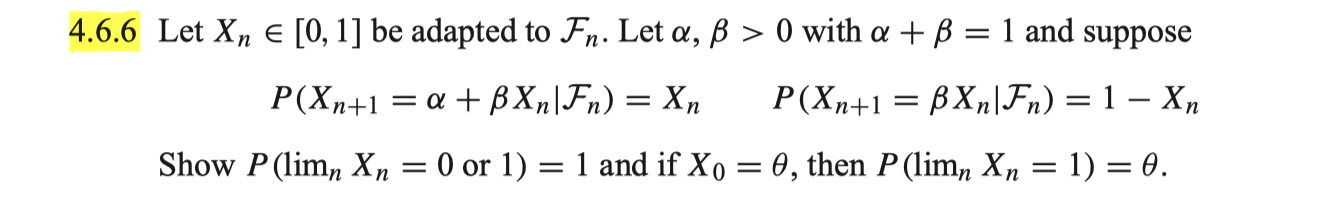
\includegraphics[width=17cm]{Exer4.6.6.png}

\begin{proof}
   $X_n\in \F_n$ and $0\leq X_n\leq 1\foranyn$ . By assumption, 
   $$X_{n=1}|\F_n = \begin{cases}
    \alpha +\beta X_n & \text{with prob. } X_n \\ \beta X_n & \text{with prob. } 1-X_n      
   \end{cases}
   $$
   Thus, we have $$E[X_{n+1}|\F_n] = (\alpha+\beta X_n)X_n +\beta X_n(1-X_n) = (\alpha+\beta)X_n = X_n $$
   Therefore, $X_n$ is a martingale. Since $X_n$ is uniformly bounded by $0$ and $1$ , we can say $X_n$ is uniformly integrable martingale. Also, $\sup_n E|X_n|\leq 1$ and by martingale convergence thm, $X_n\rightarrow X\;\,a.s.$ for some integrable $X$ . By Vitali lemma, $X_n\rightarrow X$ in $L^1$ and $E(X_n)\rightarrow E(X)$. Note that since $X_n$ is a martingale. we have $\theta = E(X_0) = E(X_1) = \cdots = E(X_n)\foranyn$ . Combining these, we have $\theta = E(X_0) = E(X_n) = E(X)\foranyn$ \\
   Now consider the case that $X_n = x$ where $0<x<1$ . Then $$ X_{n+1} |X_n =\begin{cases}
       \alpha + \beta x & \text{ with prob } x \\ \beta x & \text{ with prob } 1-x
   \end{cases} $$
   Thus , if $0<x<1$ then the sequence $X_n$ goes out of $\varepsilon$-ball contanining $x$ at the very next step $X_{n+1}$ . Therefore, the limit $X$ cannot have value $x \in (0,1)$ . \\ On the other hand, if $X_n = 0 $ then $$X_{n+1}|X_n =\begin{cases}
       \alpha & \text{ with prob } 0 \\ 0 & \text{ with prob } 1 
   \end{cases} \;= 0\;\,a.s.$$ Else, if $X_n = 1$ then $$X_{n+1}|X_n =\begin{cases}
    \alpha+\beta =1 & \text{ with prob } 1 \\ \beta & \text{ with prob } 0  
\end{cases} \;= 1\;\,a.s.$$ Therefore $X = 0$ or $1\;\,a.s.$ and $\theta =  E(X) = 0 \cdot P(X=0) + 1 \cdot P(X=1)$ so $P(X=1) =\theta$
\end{proof}

\vspace{1cm}

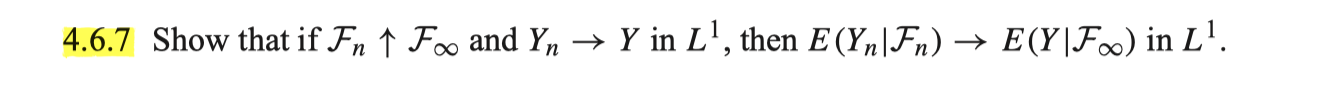
\includegraphics[width=17cm]{Exer4.6.7.png}

\begin{proof}
    We want to show the $L^1$ convergence i.e. $$E|E(Y_n |\F_n) - E(Y |\F_\infty) |\rightarrow 0 $$
    Note that by triangle inequality, we have
    $$E|E(Y_n |\F_n) - E(Y |\F_\infty) | \leq E|E(Y_n|\F_n)-E(Y|\F_n)| + E|E(Y|\F_n) - E(Y|\F_\infty)| $$
    By Levy's thm, $E(Y|\F_n) \rightarrow E(Y|\F_\infty)$ in $L^1$ so that $E|E(Y|\F_n) - E(Y|\F_\infty)|\rightarrow 0 $ \\
    Also, $$E|E(Y_n|\F_n)-E(Y|\F_n)| \leq E[E[|Y_n-Y| \big| \F_n]]= E|Y_n-Y|\rightarrow 0 $$ by the assumption that $Y_n \rightarrow Y$ in $L^1$ . Therefore $$ E|E(Y_n |\F_n) - E(Y |\F_\infty) | \rightarrow 0$$ In other words, $E(Y|\F_n)\rightarrow E(Y|\F_\infty)$ in $L^1$
\end{proof}

\vspace{1cm}

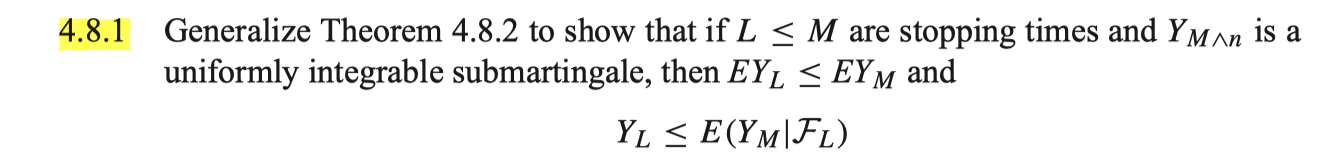
\includegraphics[width=17cm]{Exer4.8.1.png}

\begin{proof}
    We can prove this thm on four steps.
    \begin{enumerate}
        \item $E(Y_0)\leq E(Y_N)\leq E(Y_\infty)$ for any stopping time $N$ \\
        For uniformly integrable submartingale $Y_n$, we have $Y_n\rightarrow Y_\infty\;\,a.s.$ for some integrable r.v. $Y_\infty$ . Also, for a stopping time $N$, $X_n = Y_{N\wedge n}$ is also a uniformly integrable submartingale so that $X_n\rightarrow X_\infty\;\,a.s.$ for some integrable r.v. $X_\infty$ . Note that $X_\infty = Y_N\;\,a.s.$ (This is derived when we consider two cases where $N=\infty$ and $N<\infty$) . Applying Vitali lemma to both $Y_n\rightarrow Y_\infty$ and $Y_{N\wedge n}\rightarrow Y_N$ , we have $E(Y_n) \rightarrow E(Y_\infty)$ and $E(Y_{N\wedge n})\rightarrow E(Y_N)$ . Using bounded optional stopping thm, we have $$ E(Y_0) \leq E(Y_{N\wedge n}) \leq E(Y_n)$$ Taking $n\rightarrow \infty$ , we have $$ E(Y_0) \leq E(Y_N) \leq E(Y_\infty)$$
        \item $E(Y_L)\leq E(Y_M)$ given $L\leq M$ \\
        For uniformly integrable submartingale $Y_n$, we have $Y_n\rightarrow Y_\infty\;\,a.s.$ for some integrable r.v. $Y_\infty$ . $X_n = Y_{M\wedge n}$ is also a uniformly integrable submartingale so that $X_n\rightarrow X_\infty\;\,a.s.$ for some integrable r.v. $X_\infty$ . Note that $X_\infty = Y_M\;\,a.s.$ By the result of the first step, we have $$ E(X_0) \leq E(X_L) \leq E(X_\infty) $$ Since $X_L = Y_{M\wedge L}=Y_L$ and $X_\infty = Y_M\;\,a.s.$ we have $$E(Y_L) \leq E(Y_M)$$
        \item If $A\in \F_L$ then $N = L\cdot I_A + M\cdot I_{A^C}$ is a stopping time. \\ This is illustrated in exercise 4.4.3 of homework 2
        \item Show $E[Y_L I_A] \leq E[Y_M I_A] \quad \forall \; A\in \F_L$ \\ This is illustrated in exercise 4.4.4 of homework 2
    \end{enumerate}
\end{proof}

\clearpage

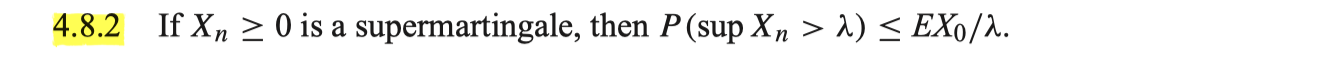
\includegraphics[width=17cm]{Exer4.8.2.png}

\begin{proof}
    We have learned in class that for nonnegative supermartingale $X_n$ , if $N$ is a stopping time then $E(X_0)\geq E(X_N)$ . Note that $N= \inf\{n : X_n >\lambda\}$ is a stopping time. On $(N<\infty)$ , we have $X_N >\lambda$ so $$X_NI(N<\infty) \geq \lambda I(N<\infty)\quad \quad  E[X_N I(N<\infty)]\geq \lambda P(N<\infty)$$ Since $X_n\geq 0$ , we get $E(X_0)\geq E(X_N) \geq E[X_N I(N<\infty)]\geq \lambda P(N<\infty)$ . Hence $$P(N<\infty) \leq \frac{E[X_0]}{\lambda}$$ Note that $$(N<\infty) = (\{n : X_n>\lambda\}\neq \phi) = (X_n > \lambda \text{ for some } n\in \N) = (\sup_n X_n >\lambda)$$ Therefore, we can conclude that $$P(\sup_nX_n>\lambda)\leq \frac{E[X_0]}{\lambda} $$
\end{proof}

\vspace{1cm}

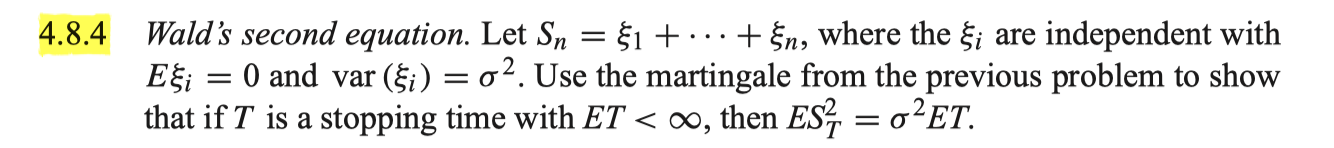
\includegraphics[width=17cm]{Exer4.8.4.png}

\begin{proof}
    As we can see in the example 4.2.2 in the textbook, $M_n = S_n^2 -n\sigma^2$ is a martingale . Since $T$ is a stopping time , $M_{T\wedge n}$ is also a martingale . Let $P_n = M_{T\wedge n}$ . Then $E(P_1) = E(P_n)$ by the property of martingale. 
    $$E(P_1) = E(M_1) = E(S_1^2 - \sigma^2) = E(\xi_1^2 - \sigma^2) = 0 $$
    $$E(P_n) = E(M_{T\wedge n}) = E[S_{n\wedge T}^2 -(n\wedge T)\sigma^2]$$
    Thus we have $E[S_{T\wedge n}^2] = \sigma^2 E[T\wedge n]\foranyn$ . Note that $E(T)<\infty$ assumption implies that $T<\infty\;\,a.s.$ Thus $S_{T\wedge n}\rightarrow S_T\;\,a.s.$ Also, since $T\wedge n \nearrow T$ and $E[T\wedge n]\nearrow E[T]$ by MCT, we get $$\sup_n E[S_{T\wedge n}^2] = \sigma^2 \sup_nE[T\wedge n] = \sigma^2 E[T]<\infty $$ Hence, we have $\sup_n E[S_{T\wedge n}^2]<\infty$ . Note that $S_n$ is also a martingale so that $S_{T\wedge n}$ is a martingale too. By martingale $L^p$ convergence thm, $S_{T\wedge n}\rightarrow S_T\;\,a.s.$ and in $L^2$ . This $L^2$ convergence gives us the fact that $E[S_{T\wedge n}^2]\rightarrow E[S_T^2]$ . Therefore, taking $n\rightarrow \infty$ for $E[S_{T\wedge n}^2] = \sigma^2 E[T\wedge n]\foranyn$  , we finally get $$E[S_T^2]=\sigma^2 E[T] $$
\end{proof}

\clearpage
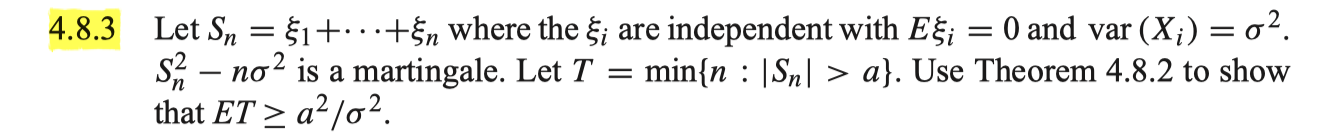
\includegraphics[width=17cm]{Exer4.8.3.png}

\begin{proof}
    Notice that $T$ is a stopping time. If $E(T)=\infty$ then the inequality trivially holds so assume that $E(T)<\infty$ . Then, by the Wald's second equation we proved in the previous exercise, we have $E[S_T^2] = \sigma^2 E[T]$ . Observe that on $(T<\infty)$ , we get $S_T^2>a^2$ . Hence we have $$E[S_T^2] \geq E[S_T^2 I(T<\infty)]\geq a^2E[I(T<\infty)] = a^2 P(T<\infty)$$ The assumption $E[T]<\infty$ implies that $T<\infty \;\,a.s.$ thus $P(T<\infty)=1$ . Therefore, $$E[T]= E[S_T^2]/ \sigma^2\geq a^2/\sigma^2 $$
\end{proof}

\vspace{1cm}

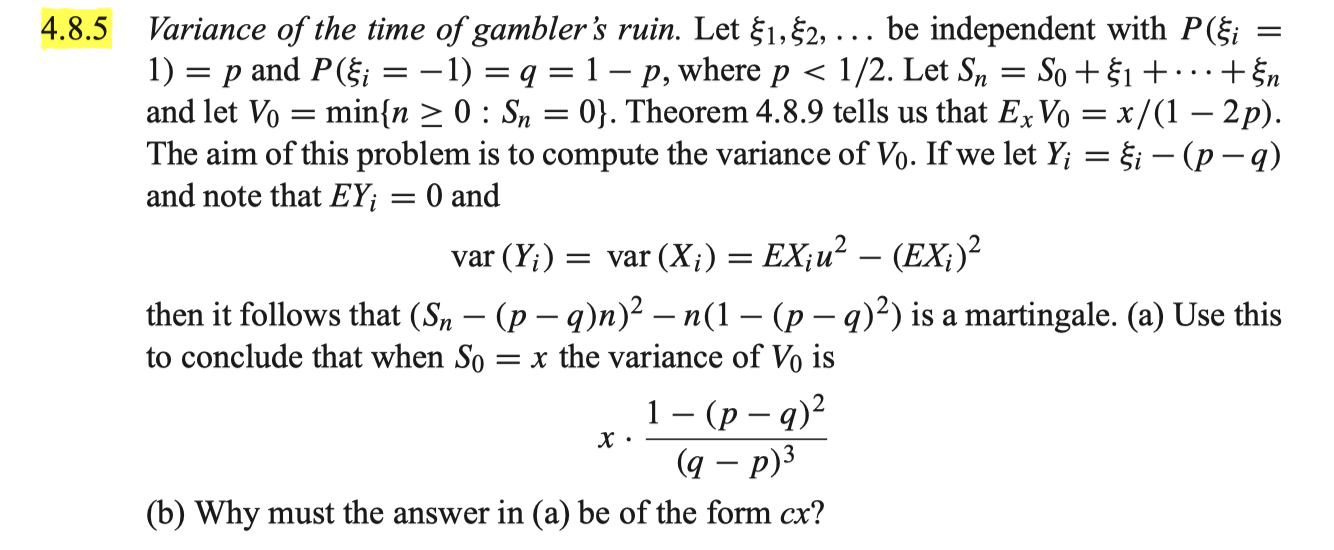
\includegraphics[width=17cm]{Exer4.8.5.png}

\begin{proof}
    Here $x>0$ is assumed. (Otherwise, variance becomes negative which is nonsense)\\
    Note that $E[Y_1] = 0$ and $Var[Y_1] = 1 - (p-q)^2$ . $S_n - n(p-q) = S_0 + Y_1+\cdots + Y_n$ . We have observed that $S_n^2 -n\sigma^2$ is martingale provided $S_n = \xi_1+\cdots+\xi_n$ and $\xi_i$ i.i.d. with $E[\xi_1]=0$ and $Var[\xi_1]\sigma^2$ Here, $Y_i$ plays a role of $\xi_i$ in the sense that it has zero mean. Thus, $$(S_n - n(p-q))^2 -n(1-(p-q))^2 $$ is a martingale. In the lecture, we have learned that $T_a<\infty \;\,a.s.$ for $a<0$ . Here, it is replaced by $V_0<\infty \;\,a.s.$ for $0<x$ . (The former has starting point $0$ and target point $a$, while the latter has starting point $x$ and target point $0$) . Since $E[V_0] = \frac{x}{1-2p}<\infty$ , we can apply Wald second identity. \\ Let $\tilde S_n = Y_1+\cdots+Y_n = S_n - n(p-q)-S_0$ . Applying Wald second identity, we have $$E[\tilde{S}_{V_0}^2] = (1-(p-q)^2)E[V_0] $$. Plugging in $\tilde S_n =S_n - n(p-q)-S_0$ and $E[V_0]=\frac{x}{q-p}$ , we get
    $$E\big[(S_{V_0} - V_0(p-q)-x)^2 \big]= (1-(p-q)^2)\frac{x}{q-p} $$ Note that $S_{V_0}=0\;\,a.s.$ since $V_0<\infty \;\,a.s.$ . Thus , we can derive that 
    \begin{align*}
        E\big[(S_{V_0} - V_0(p-q)-x)^2 \big]&= E\big[(-V_0(p-q)-x)^2\big] = E\big[(V_0(p-q)+x)^2\big]\\ 
        &= E\big[\big\{(p-q)\big(V_0+\frac{x}{p-q} \big)\big\}^2\big] = (q-p)^2 E\big[\big(V_0 -\frac{x}{q-p}\big)^2\big] \\ &= (q-p)^2 E[\{V_0 -E(V_0)\}^2] = (q-p)^2 Var(V_0)
    \end{align*}
    Therefore, we have
    $$Var(V_0)= \frac{x(1-(p-q)^2)}{(q-p)^3} $$
\end{proof}

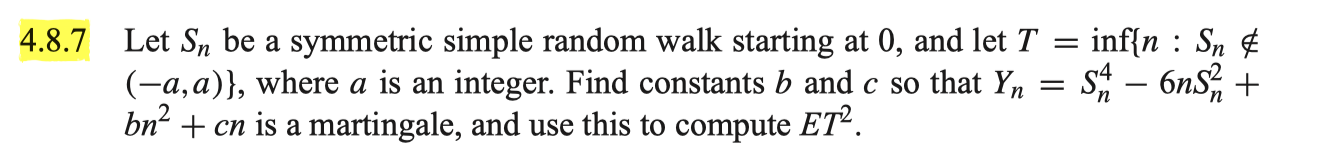
\includegraphics[width=17cm]{Exer4.8.7.png}

\begin{proof}
    $S_n = \xi_1 + \cdots + \xi_n$ with $\xi_i$ i.i.d. where $P(\xi_1 = 1) = P(\xi_1 = -1)=0.5$ . $E(\xi_1)=0$ and $Var(\xi_1)=1$ . Note that $S_n^2 - n$ is a martingale. Since $T$ is a stopping time, $S_{T\wedge n}^2 -(T\wedge n)$ is a martingale . $$E[S_{T\wedge n}^2 -(T\wedge n)] = E[S_1^2 -1] = E[\xi_1^2]-1 =0$$ Hence $E[S_{T\wedge n}^2] = E[T\wedge n]\foranyn$ . Here, we shall claim that $T<\infty\;\,a.s.$ \\ Note that wherever $S_n$ lies between $(-a, a)$ , if we have $2a$ consecutive steps of size $+1$ then we will exit the interval $(-a, a)$ . It can be written as $$(T>m\cdot 2a)\subset (m \text{ times fail of } ``2a \text{ consecutive steps of size +1}'') $$ 
    $$P(T>2ma) \leq \bigg(1-\big(\frac{1}{2}\big)^{2a} \bigg)^m $$
    Taking $m\rightarrow \infty$ , we have $P(T=\infty) = 0$ . Hence, $T<\infty\;\,a.s.$ Thus $S_{T\wedge n}\rightarrow S_T\;\,a.s.$ and $S_{T\wedge n}^2\rightarrow S_T^2\;\,a.s.$  Observe that $S_T^2=a^2\;\,a.s.$ and $|S_{T\wedge n}^2|\leq a^2$ so that applying BCT , we get $$E[S_{T\wedge n}^2]\rightarrow E[S_T^2]=E[a^2]=a^2 $$ Also, by MCT , $E[T\wedge n]\nearrow E[T]$ . From the equality $E[S_{T\wedge n}^2]=E[T\wedge n]\foranyn$ , we can conclude that $E[T]=a^2$
    Now, we shall calculate $E[Y_{n+1}|\F_n]=Y_n$ to make $Y_n$ be a martingale.
    \begin{align*}
        E[Y_{n+1}|\F_n] &= E[(S_n+\xi_{n+1})^4-6(n+1)(S_n+\xi_{n+1})^2+b(n+1)^2+c(n+1)|\F_n] \\ &= S_n^4 + 6S_n^2 -6(n+1)S_n^2 -6(n+1) + bn^2 +b(2n+1)+cn +c \\ &= S_n^5-6nS_n^2 +bn^2 +cn +(2b-6)n +(b+c-5) =Y_n
    \end{align*}
    To satisfy the last equation, $b=3$ and $c=2$ is the right choice. Since $Y_{T\wedge n}$ is a martingale , $E[Y_1]=E[Y_{T\wedge n}]$ and we have 
    $$E[S_{T\wedge n}^4]-6E[(T\wedge n)S_{T\wedge n}^2]+3E[(T\wedge n)^2]+2E[T\wedge n]=0 $$
    Taking $n\rightarrow$ , by DCT and MCT , we get 
    $$a^4-6a^2 E[T]+3E[T^2]+2E[T]=0 $$
    Using $E[T]=a^2$ , we get $E[T^2]=(5a^4-2a^2)/3$
\end{proof}

\end{document}
